\chapter{Empirical Results and Discussion}

\label{ch:empirical-results-and-discussion}

This chapter reports the empirical performance of every loss function that enters the final recommendation. All numbers quoted here are traceable to a single source-of-truth evidence map; each caption records the evaluation window, the seed set, and the underlying artifact path so the reader can audit the claim.

The structure of the chapter mirrors the empirical pipeline rather than the order in which the experiments were carried out. Section~5.1 restates the shared evaluation protocol. Sections~5.2--5.3 present same-window single-seed comparisons (baseline losses and the hybrid A/M sweep, both at seed 42); within each comparison table, the loss function is the only varying factor. Sections~5.4--5.5 move to multi-seed evidence on the M2-robust family and the broader $\alpha/\beta/\lambda$ sweeps, which form the basis of the final recommendation; cross-phase comparisons differ in additional dimensions (\S5.7). Section~5.6 discusses a loss-component normalisation probe. Section~5.7 scopes the boundary of cross-phase comparison claims. Section~5.8 synthesises the headline findings and bridges to the conclusion.

\section{Evaluation protocol recap}

\label{sec:evaluation-protocol-recap}

All experiments use the protocol defined in Chapter~3 \S3.4 and the X1 feature input from Chapter~4. The key operational parameters are: train \texttt{1990-01..1994-12} (60 months), test \texttt{1995-01..1996-12} (24 months), MLP[64,32,16]+ReLU+dropout 0.2, batch size 1024, 20 epochs, top/bottom 10\% signal-tilted long-short portfolio with 5\% per-name cap. Sharpe is annualised as $\sqrt{12} \cdot \bar r / \sigma_r$. Single-seed tables (\S5.2--\S5.3) use seed 42; multi-seed tables (\S5.4--\S5.6) use three seeds per row. Source paths are listed in each table caption; full reproduction commands are in Appendix~B.

\section{Phase 1: Baseline loss comparison (24 months, seed 42)}

\label{sec:phase1-baseline-loss-comparison}

Table~\ref{tab:baseline-loss-comparison} reports the main baseline-loss comparison under the static 24-month window at seed 42. The seven rows cover the traditional regression losses (MSE, MedSE), the absolute-loss family (MADL, GMADL, IMADL), and the two hybrid multiplicative variants (\texttt{hybrid\_mul\_m1}, \texttt{hybrid\_mul\_m2}) that will be extended in \S5.3.

\begin{table}[H]
\centering
\caption{Baseline loss comparison. Static train \texttt{1990-01..1994-12}, test \texttt{1995-01..1996-12}, seed 42, MLP[64,32,16]+ReLU+dropout 0.2, X1, batch 1024, 20 epochs, top/bottom 10\% with 5\% per-name cap. Source: see Appendix~B \SB.4.}
\label{tab:baseline-loss-comparison}
\begin{tabular}{cccccc}
\toprule
Loss & Sharpe & Cum.\ return & Avg R$^2$ & Avg monthly LS & Monthly LS std \\
\midrule
MSE & $-0.4643$ & $-0.1125$ & $-102.1787$ & $-0.004422$ & $0.032989$ \\
MedSE & $0.0932$ & $0.0060$ & $-2\,297\,042.29$ & $0.001214$ & $0.045124$ \\
MADL & $-0.3058$ & $-0.0756$ & $-4.15 \times 10^{9}$ & $-0.002794$ & $0.031653$ \\
GMADL & $0.2025$ & $0.0279$ & $-7.02 \times 10^{9}$ & $0.001429$ & $0.024449$ \\
IMADL & $-0.3732$ & $-0.0944$ & $-106.5114$ & $-0.003578$ & $0.033211$ \\
\texttt{hybrid\_mul\_m1} & $0.4435$ & $0.0509$ & $-4.7942$ & $0.002215$ & $0.017302$ \\
\texttt{hybrid\_mul\_m2} & $-0.0017$ & $-0.0032$ & $-1.0298$ & $-0.000008$ & $0.016096$ \\
\bottomrule
\end{tabular}
\end{table}

Three observations follow from the table.

First, neither traditional regression loss yields an economically meaningful long-short portfolio at this single seed. MSE is strongly negative in both Sharpe and cumulative return, and MedSE is only nominally positive (Sharpe $0.0932$, cumulative return $+0.60\%$ over 24 months). This stands in contrast to earlier preliminary six-month checks in which MedSE appeared to dominate; under the same protocol extended to 24 months at seed 42, the MedSE advantage vanishes and the headline numbers belong in \S5.4 to the multi-seed M2-robust family, not to MedSE.

Second, the absolute-loss family produces extremely negative average R$^2$ values ($-4.15 \times 10^{9}$ for MADL and $-7.02 \times 10^{9}$ for GMADL). This does not indicate that the portfolio signal is uninformative -- GMADL yields a positive Sharpe ($0.2025$), second among the non-hybrid baselines (behind only \texttt{hybrid\_mul\_m1}). Rather, the point-prediction scale has diverged from the realised-return scale: under a direction/magnitude-weighted objective the MLP produces predictions that are orders of magnitude away from the realised return in absolute terms. Because the long-short construction uses only the cross-sectional rank of the predictions, portfolio performance is decoupled from calibration quality. This decoupling is central to interpreting the rest of the chapter: absolute-loss-style variants should be evaluated by their ranked portfolio metrics (Sharpe, cumulative return) and, where multi-seed evidence exists, CV across seeds, rather than by R$^2$.

Third, among baseline losses, \texttt{hybrid\_mul\_m1} yields the best single-seed Sharpe at $0.4435$, nearly twice the next-highest. Its cumulative return over 24 months is $+5.09\%$ and its monthly LS standard deviation is the lowest of the set at $0.017302$, suggesting that combining a directional-prediction term with a rank-preserving term produces a more stable long-short signal than either an MSE or an MADL-style term alone. This result motivates the hybrid sweep in \S5.3.

Table~\ref{tab:baseline-loss-comparison} is a same-window single-seed comparison. It is informative for ranking loss families at a fixed seed but cannot support statements about robustness to seed perturbation. Seed-sensitivity claims are reserved for \S5.4 and \S5.5.

\begin{figure}[H]
\centering

\includegraphics[width=0.9\textwidth]{figures/fig5_1_baseline_comparison.png}
\caption[Baseline loss comparison: cumulative return and Sharpe]{Baseline loss comparison. Left: monthly cumulative long-short return per loss over 1995-01..1996-12; \texttt{hybrid\_mul\_m1} is drawn bold with markers. Right: annualised Sharpe sorted descending, with \texttt{hybrid\_mul\_m1} hatched in deep navy as the seed-42 peak. Seed 42, cap05 portfolio, MLP[64,32,16]+ReLU+dropout 0.2, X1, batch 1024, 20 epochs.}
\label{fig:baseline-loss-comparison}
\end{figure}

\section{Phase 2: Hybrid A/M variant sweep (24 months, seed 42)}

\label{sec:phase2-hybrid-am-sweep}

This phase extends the two hybrid multiplicative variants of \S5.2 into a parameterised family of nine variants (additive A1--A5 and multiplicative M1--M4; see Chapter~3 \S3.3 for definitions). All nine runs use the same static window, feature set, and portfolio construction as Table~\ref{tab:baseline-loss-comparison}; only the loss specification changes.

\begin{table}[H]
\centering
\caption{Phase 2 additive (A1--A5) and multiplicative (M1--M4) variants. Static train \texttt{1990-01..1994-12}, test \texttt{1995-01..1996-12}, seed 42, same model / feature / portfolio configuration as Table~\ref{tab:baseline-loss-comparison}. Source: see Appendix~B \SB.4.}
\label{tab:phase2-variants}
\begin{tabular}{ccccc}
\toprule
Variant & Loss ID & Sharpe & Cum.\ return & Avg R$^2$ \\
\midrule
A1 & \texttt{hybrid\_add\_a1} & $0.1241$ & $0.0133$ & $-2\,105.95$ \\
A2 & \texttt{hybrid\_add\_a2} & $0.2173$ & $0.0450$ & $-484.75$ \\
A3 & \texttt{hybrid\_add\_a3} & $\mathbf{0.5738}$ & $\mathbf{0.0813}$ & $-1\,383.64$ \\
A4 & \texttt{hybrid\_add\_a4} & $0.2311$ & $0.0463$ & $-11\,229.79$ \\
A5 & \texttt{hybrid\_add\_a5} & $-0.4110$ & $-0.2080$ & $-507\,162.38$ \\
M1 & \texttt{hybrid\_mul\_m1} & $\mathbf{0.4435}$ & $\mathbf{0.0509}$ & $-4.79$ \\
M2 & \texttt{hybrid\_mul\_m2} & $-0.0017$ & $-0.0032$ & $-1.03$ \\
M3 & \texttt{hybrid\_mul\_m3} & $-0.9691$ & $-0.0903$ & $-0.44$ \\
M4 & \texttt{hybrid\_mul\_m4} & $-0.3440$ & $-0.0409$ & $-0.06$ \\
\bottomrule
\end{tabular}
\end{table}

The additive family peaks at A3 with Sharpe $0.5738$ and cumulative return $+8.13\%$; A4 and A2 are second-tier; A5 collapses as the added term overwhelms the base MSE contribution. The multiplicative family peaks at M1 with Sharpe $0.4435$ (identical to its Table~\ref{tab:baseline-loss-comparison} row because the runner and configuration are unchanged); M2 through M4 degrade monotonically on Sharpe.

A few interpretive notes matter for later sections. (i)~At seed 42, A3 slightly outperforms M1 on Sharpe and cumulative return, yet the multiplicative family is the one that Phase 3 extends into the M2-robust $\gamma$ parameterisation. The rationale for that design choice is discussed in Chapter~3; the empirical support is that A3's R$^2$ magnitude ($-1\,383.64$, driven by the additive MSE term being dominated by a scale-insensitive accuracy term) offers less interpretable control than the M-family, whose R$^2$ remains within a small single-digit range. (ii)~Seed-42 peaks do not survive seed perturbation uniformly. In \S5.4 the M2-robust $\gamma$ sweep is evaluated across three seeds and the ordering of mean Sharpe does not match the single-seed ordering in this table. Consequently, the Phase~1.5 rows should be read as \emph{motivation} for the Phase~2 design, not as a final variant ranking.

The additive family is not carried further into multi-seed robustness in this report. The final recommendation in \S5.8 draws on the multi-seed evidence for the M2-robust family (\S5.4) and on the integrated cross-variant sweep (\S5.5).

\begin{figure}[H]
\centering

\includegraphics[width=0.9\textwidth]{figures/fig5_2_phase15_variants.png}
\caption[Phase 2 hybrid variants: additive A1--A5 and multiplicative M1--M4]{Phase 2 hybrid variants. Horizontal grouped bars showing annualised Sharpe for (a) additive A1--A5 (warm palette) and (b) multiplicative M1--M4 (cool palette); seed-42 peaks A3 and M1 are hatched in deep red/navy and their Sharpe values are rendered in dark-red bold. Same runner/feature/portfolio/architecture as Table~\ref{tab:baseline-loss-comparison}.}
\label{fig:phase2-variants}
\end{figure}

\section{Phase 3a: Multi-seed $\gamma$ refinement}

\label{sec:phase3a-gamma-refinement}

Phase~2 introduces an explicit robustness parameter $\gamma$ into the multiplicative hybrid M2 variant, producing the family of \texttt{m2\_robust\_gamma\{0.03, 0.05, 0.07, 0.10, 0.15\}} losses. Each variant is run across three random seeds using the same 24-month static window and the 5\% per-name portfolio cap (\texttt{cap05}). The purpose is to decouple the seed-42 ranking of \S5.3 from a claim about the expected performance of the loss under seed perturbation.

Sharpe stability is reported as the coefficient of variation $\mathrm{CV} = \sigma_S / |\mu_S|$, where $\mu_S$ and $\sigma_S$ are the cross-seed mean and standard deviation of the annualised Sharpe (same $\sqrt{12}$-annualised convention as \S5.1 and \S5.2). Lower CV implies lower relative seed sensitivity.

\begin{table}[H]
\centering
\caption{Phase 3a $\gamma$ refinement, multi-seed (3 seeds per row). Static train \texttt{1990-01..1994-12}, test \texttt{1995-01..1996-12}, \texttt{cap05} portfolio cap. Each row aggregates three seeds. Source: see Appendix~B \SB.4.}
\label{tab:gamma-refinement}
\begin{tabular}{cccccc}
\toprule
Loss & Runs & Sharpe mean & Sharpe std & Cum.\ return mean & CV \\
\midrule
\texttt{m2\_robust\_gamma03} & 3 & $0.3234$ & $0.3418$ & $0.0818$ & $1.0570$ \\
\texttt{m2\_robust\_gamma05} & 3 & $0.7054$ & $0.1488$ & $0.2392$ & $0.2109$ \\
\texttt{m2\_robust\_gamma07} & 3 & $\mathbf{0.9156}$ & $0.1655$ & $\mathbf{0.2799}$ & $\mathbf{0.1808}$ \\
\texttt{m2\_robust\_gamma10} & 3 & $1.0043$ & $0.5638$ & $0.2368$ & $0.5613$ \\
\texttt{m2\_robust\_gamma15} & 3 & $0.8163$ & $0.3724$ & $0.2277$ & $0.4562$ \\
\bottomrule
\end{tabular}
\end{table}

\vspace{-1em}
\begin{figure}[H]
\centering

\includegraphics[width=0.9\textwidth]{figures/fig5_3_gamma_refinement.png}
\caption[Phase 3a $\gamma$ refinement: multi-seed Sharpe and stability]{Phase 3a $\gamma$ refinement: multi-seed Sharpe and stability. Left: cross-seed mean annualised Sharpe with $\pm 1$ std error bars (3 seeds per $\gamma$); light vertical bars indicate the min--max range. Right: coefficient of variation CV $= \sigma / |\mu|$. Evaluation window \texttt{1995-01..1996-12}, \texttt{cap05} portfolio cap.}
\label{fig:gamma-refinement}
\end{figure}

Figure~\ref{fig:gamma-tuning-curve} presents the same $\gamma$ sweep as a continuous tuning curve, adding a third panel that reports the mean monthly long-short return standard deviation across seeds. The three-panel view makes the trade-off explicit: \texttt{gamma07} sits at the stability peak on all three dimensions simultaneously -- it does not merely minimise CV while sacrificing Sharpe, nor does it minimise portfolio volatility at the cost of return. \texttt{gamma10} is visibly higher on the Sharpe axis but also higher on both the CV and the volatility axes, confirming that its apparent Sharpe advantage comes with a measurable increase in prediction-level variance.

\begin{figure}[H]
\centering
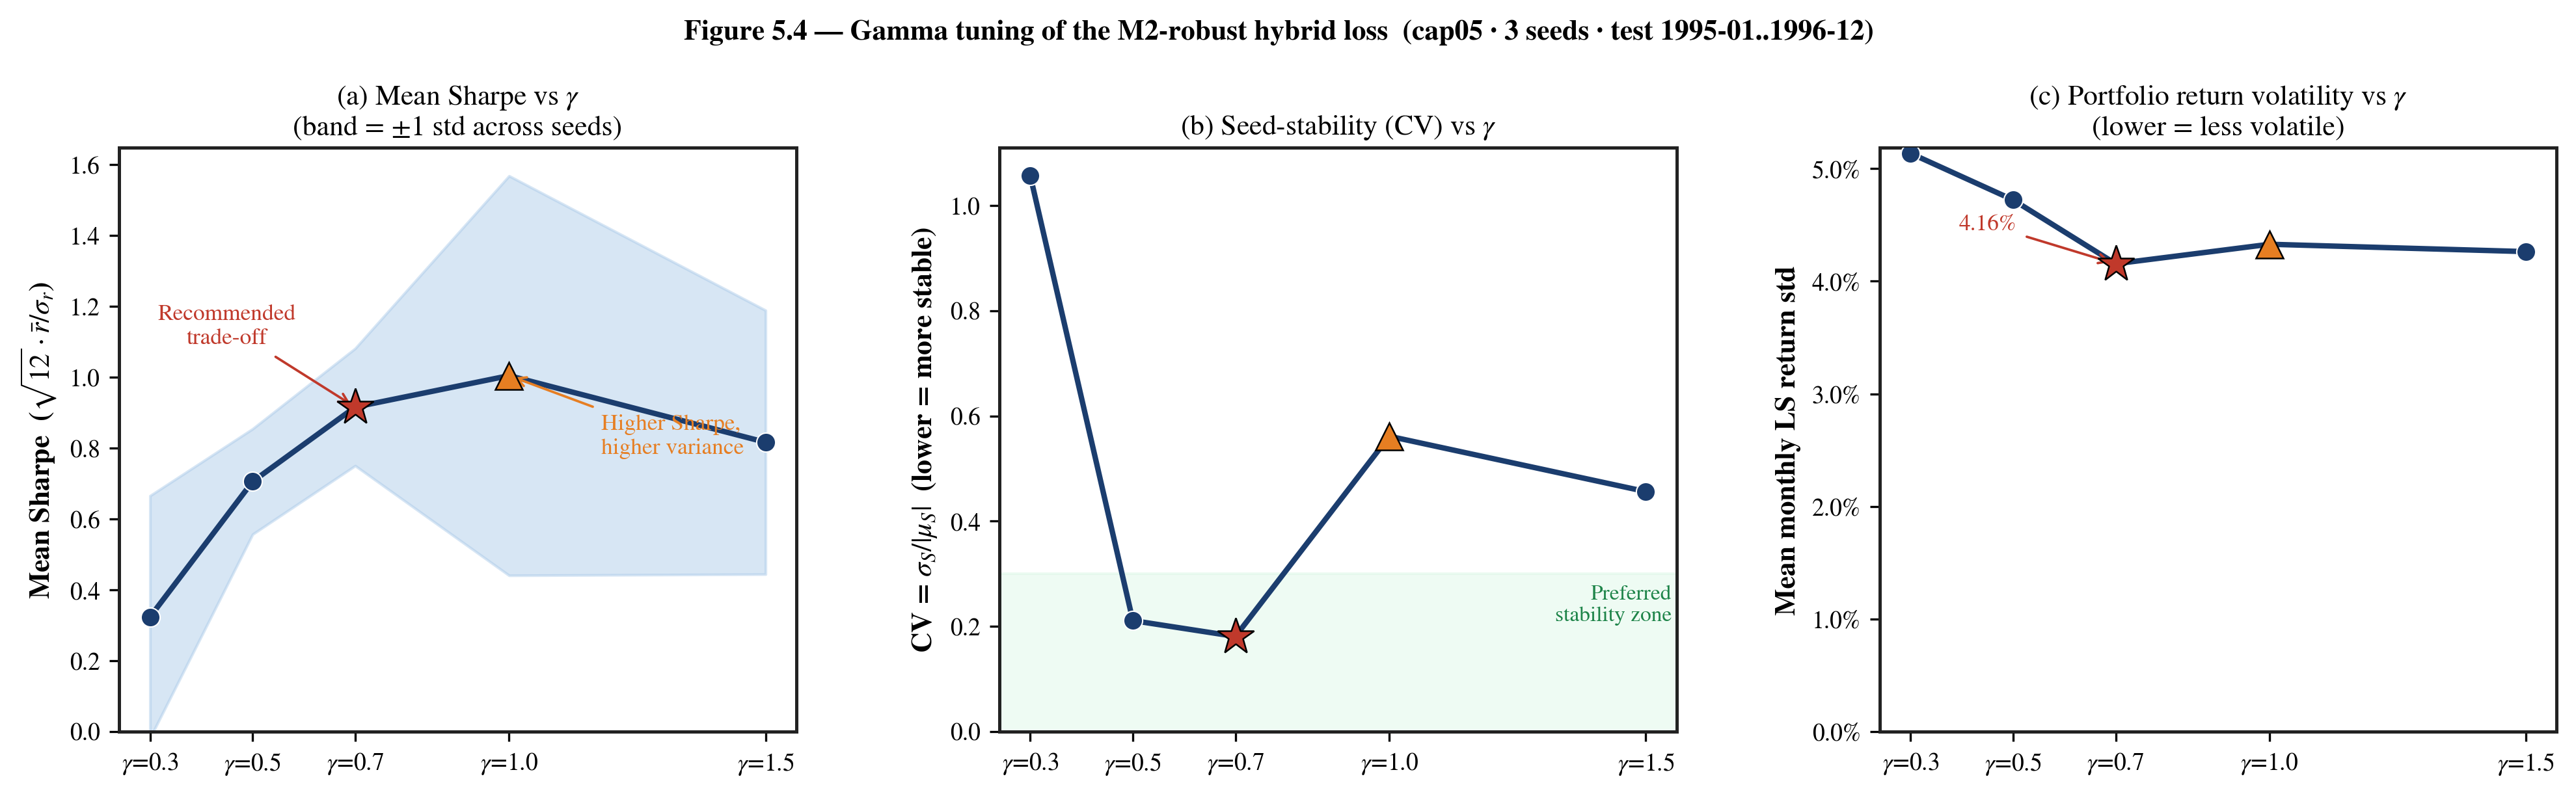
\includegraphics[width=0.9\textwidth]{figures/fig5_4_gamma_tuning_curve.png}
\caption[$\gamma$ tuning curve: Sharpe, stability, and portfolio volatility]{$\gamma$ tuning curve: Sharpe, stability, and portfolio volatility. Panel~(a): mean annualised Sharpe vs $\gamma$ with $\pm 1$ std band across 3 seeds. Panel~(b): cross-seed CV vs $\gamma$; green shading marks the preferred stability zone (CV $\leq 0.30$). Panel~(c): mean monthly long-short return standard deviation vs $\gamma$ -- a direct measure of portfolio-level variance. Red star: \texttt{gamma07} (recommended); orange triangle: \texttt{gamma10} (higher Sharpe, higher variance). Evaluation window \texttt{1995-01..1996-12}, \texttt{cap05}, 3 seeds per row.}
\label{fig:gamma-tuning-curve}
\end{figure}

Three findings follow from Table~\ref{tab:gamma-refinement}.

First, \texttt{m2\_robust\_gamma07} provides the best Sharpe-vs-stability trade-off in the $\gamma$ sweep. Its mean Sharpe of $0.9156$ is within $9\%$ of the highest mean ($1.0043$ for \texttt{gamma10}), while its coefficient of variation is the lowest among the non-collapsed variants at $0.1808$ -- roughly one-third of the CV of \texttt{gamma10}. Its mean cumulative return of $+27.99\%$ over 24 months is the largest in the table. Across three seeds, its minimum Sharpe is $0.7532$; no seed in the run produces a negative Sharpe.

Second, \texttt{m2\_robust\_gamma10} has the highest mean Sharpe ($1.0043$) but also the highest CV among the strong variants ($0.5613$). Its per-seed Sharpe range is wide ($0.4587$ to $1.5847$). Interpreted cautiously, \texttt{gamma10} is a variant whose \emph{best} seed produces the best Sharpe of the entire $\gamma$ family, but whose \emph{average} seed has not materially improved on \texttt{gamma07}. A recommendation that selects the variant with the highest mean Sharpe should therefore come with an explicit seed-sensitivity caveat.

Third, the $\gamma$ schedule exhibits a non-monotone relationship with Sharpe stability. \texttt{gamma03} collapses almost entirely (CV $1.0570$, minimum Sharpe negative), and \texttt{gamma15} -- past the stability peak -- also degrades sharply in CV ($0.4562$) even though its mean Sharpe remains respectable ($0.8163$). The stability peak near $\gamma = 0.07$ is thus an internal optimum of the robust component rather than the endpoint of a monotone trend. This is consistent with the design intent of the robust modifier: too little robustness under-weights the rank-preserving term; too much robustness flattens the loss surface and re-injects seed-level noise into the learned weights.

On this evidence alone, \texttt{m2\_robust\_gamma07} is the best-supported candidate for the primary recommendation in \S5.8. The fuller comparison in \S5.5 -- where \texttt{gamma07} is evaluated against $\alpha$- and $\beta$-sweep variants from other families -- confirms this ordering.

\section{Phase 3b: Integrated $\alpha$, $\beta$, and $\lambda$ sweeps}

\label{sec:phase3b-integrated-sweeps}

To rule out the possibility that the M2-robust $\gamma$ family is merely a locally good design in the hybrid-multiplicative corner of the loss space, Phase~2 also runs an integrated sweep over three other parameterised families: the IMADL-m2 $\alpha$ sweep, the IMADL-GMADL $\beta$ sweep, and an adaptive-$\lambda$ family. Table~\ref{tab:integrated-summary} reports selected grouped summaries; the complete table contains further fine-grained $\gamma$ variants (\texttt{gamma001}, \texttt{gamma01}) used for locating the $\gamma$ optimum. Note that \texttt{m2\_robust\_gamma07}, the primary recommendation, is reported in Table~\ref{tab:gamma-refinement} and serves as the reference line in Figure~\ref{fig:gamma-refinement}.

Source: integrated grouped summary CSV (see Appendix~B \SB.3 for the exact branch path). All rows are 3-seed averages at \texttt{cap05} with the same 24-month window as Table~\ref{tab:gamma-refinement}.

\begin{table}[H]
\centering
\caption{Phase 2 integrated summary across $\alpha$, $\beta$, $\lambda$ families (selected rows). Static train \texttt{1990-01..1994-12}, test \texttt{1995-01..1996-12}, \texttt{cap05}, 3 seeds per row.}
\label{tab:integrated-summary}
\begin{tabular}{ccccc}
\toprule
Loss & Sharpe mean & Sharpe std & Cum.\ return mean & CV \\
\midrule
\texttt{adaptive\_lambda10} & $0.4938$ & $0.7617$ & $0.0618$ & $1.5426$ \\
\texttt{adaptive\_lambda50} & $0.2763$ & $0.1597$ & $0.0817$ & $0.5780$ \\
\texttt{adaptive\_lambda100} & $0.0955$ & $0.0343$ & $0.0021$ & $0.3591$ \\
\texttt{imadl\_gmadl\_beta03} & $-0.0345$ & $0.1381$ & $-0.0424$ & $4.0084$ \\
\texttt{imadl\_gmadl\_beta05} & $0.0406$ & $0.4116$ & $-0.0138$ & $10.1328$ \\
\texttt{imadl\_gmadl\_beta07} & $-0.0020$ & $0.2747$ & $-0.0409$ & $139.51$ \\
\texttt{imadl\_m2\_alpha02} & $0.1788$ & $1.1576$ & $0.2225$ & $6.4735$ \\
\texttt{imadl\_m2\_alpha03} & $0.2159$ & $0.2010$ & $0.0588$ & $0.9310$ \\
\texttt{imadl\_m2\_alpha04} & $0.3540$ & $0.0656$ & $0.0962$ & $0.1853$ \\
\texttt{imadl\_m2\_alpha05} & $0.5822$ & $0.3193$ & $0.2465$ & $0.5484$ \\
\texttt{imadl\_m2\_alpha06} & $\mathbf{0.6895}$ & $0.1685$ & $\mathbf{0.3042}$ & $\mathbf{0.2443}$ \\
\texttt{imadl\_m2\_alpha07} & $0.4024$ & $0.2466$ & $0.1036$ & $0.6128$ \\
\texttt{imadl\_m2\_alpha08} & $0.5683$ & $0.4130$ & $0.2071$ & $0.7267$ \\
\texttt{m2\_robust\_gamma001} & $0.6919$ & $0.8258$ & $0.1705$ & $1.1936$ \\
\texttt{m2\_robust\_gamma01} & $0.7470$ & $0.3937$ & $0.2718$ & $0.5270$ \\
\texttt{m2\_robust\_gamma10} & $1.0043$ & $0.5638$ & $0.2368$ & $0.5613$ \\
\bottomrule
\end{tabular}
\end{table}

\begin{figure}[H]
\centering

\includegraphics[width=0.9\textwidth]{figures/fig5_5_imadl_alpha_sweep.png}
\caption[IMADL-m2 $\alpha$ sweep vs $\gamma$ reference]{IMADL-m2 $\alpha$ sweep vs $\gamma$ reference. Left: cross-seed mean annualised Sharpe with $\pm 1$ std error bars for $\alpha \in \{0.2, \ldots, 0.8\}$; dashed horizontal lines mark the mean Sharpe of \texttt{m2\_robust\_gamma07} (red) and \texttt{m2\_robust\_gamma10} (orange) as references. Right: coefficient of variation on a log scale, with the same $\gamma$ references. Evaluation window \texttt{1995-01..1996-12}, \texttt{cap05}, 3 seeds per row. Source: integrated grouped summary CSV and $\gamma$ refinement grouped summary (see Appendix~B \SB.3 for exact paths).}
\label{fig:imadl-alpha-sweep}
\end{figure}

The IMADL-m2 $\alpha$ sweep produces a clean unimodal Sharpe curve with a peak at \texttt{alpha06} (mean Sharpe $0.6895$, cumulative return $+30.42\%$, CV $0.2443$). Below the peak, \texttt{alpha04} and \texttt{alpha05} remain competitive and, in the case of \texttt{alpha04}, even more stable (CV $0.1853$) at the cost of substantially lower mean Sharpe. Above the peak, \texttt{alpha07} and \texttt{alpha08} degrade. The peak's mean Sharpe is below the \texttt{gamma07} mean but its cumulative return is slightly higher, and its seed-sensitivity is only moderately worse. IMADL-m2 $\alpha$06 is therefore a sensible fallback for interpretations that prioritise cumulative return over volatility.

The IMADL-GMADL $\beta$ family does not produce a robust positive Sharpe across seeds. All three $\beta$ values have mean Sharpe close to zero and CV values in the single digits or larger ($\beta$07 has CV $\sim 140$, arising from a near-zero mean Sharpe). This indicates that directly composing IMADL with the GMADL exponent introduces scale instabilities similar to those observed in \S5.2 for GMADL alone, and normal $\beta$-tuning does not recover the stability of \texttt{m2\_robust\_gamma07}. No $\beta$ row is carried into the final recommendation.

The adaptive-$\lambda$ family, in which the relative weighting of the robust and directional terms is tuned during training, underperforms both in mean Sharpe and in stability. The best row in the family (\texttt{adaptive\_lambda10}) has mean Sharpe $0.4938$ but CV $1.5426$ -- the largest among the non-IMADL-m2-$\alpha$02 and non-GMADL-$\beta$ rows in Table~\ref{tab:integrated-summary} (only \texttt{imadl\_m2\_alpha02} at CV $6.4735$ and the $\beta$ family exceed it). The ordering $\lambda$10 $>$ $\lambda$50 $>$ $\lambda$100 indicates the family prefers moderate weighting, but even the best moderate setting does not reach the $\gamma$ or $\alpha$ peaks.

Combining Table~\ref{tab:gamma-refinement} and Table~\ref{tab:integrated-summary} confirms that the two best candidates in the final recommendation come from the two self-consistent peaks: \texttt{m2\_robust\_gamma07} at Sharpe $0.9156$ / CV $0.1808$, and \texttt{imadl\_m2\_alpha06} at Sharpe $0.6895$ / CV $0.2443$.

Figure~\ref{fig:sharpe-cv-frontier} places all multi-seed hybrid variants on a single Sharpe-stability plane, making the frontier structure visible. The preferred region -- high Sharpe, low CV -- is occupied exclusively by \texttt{gamma07}. \texttt{gamma10} lies outside the preferred region on the CV axis despite its higher mean Sharpe. \texttt{alpha06} lies inside the preferred region on the CV axis but below \texttt{gamma07} on the Sharpe axis. No other variant from the $\alpha$, $\beta$, or adaptive-$\lambda$ families reaches the preferred region. The frontier view confirms that the recommendation is not a local optimum within a single family but the dominant point across the full hybrid design space explored in this study.

\begin{figure}[H]
\centering
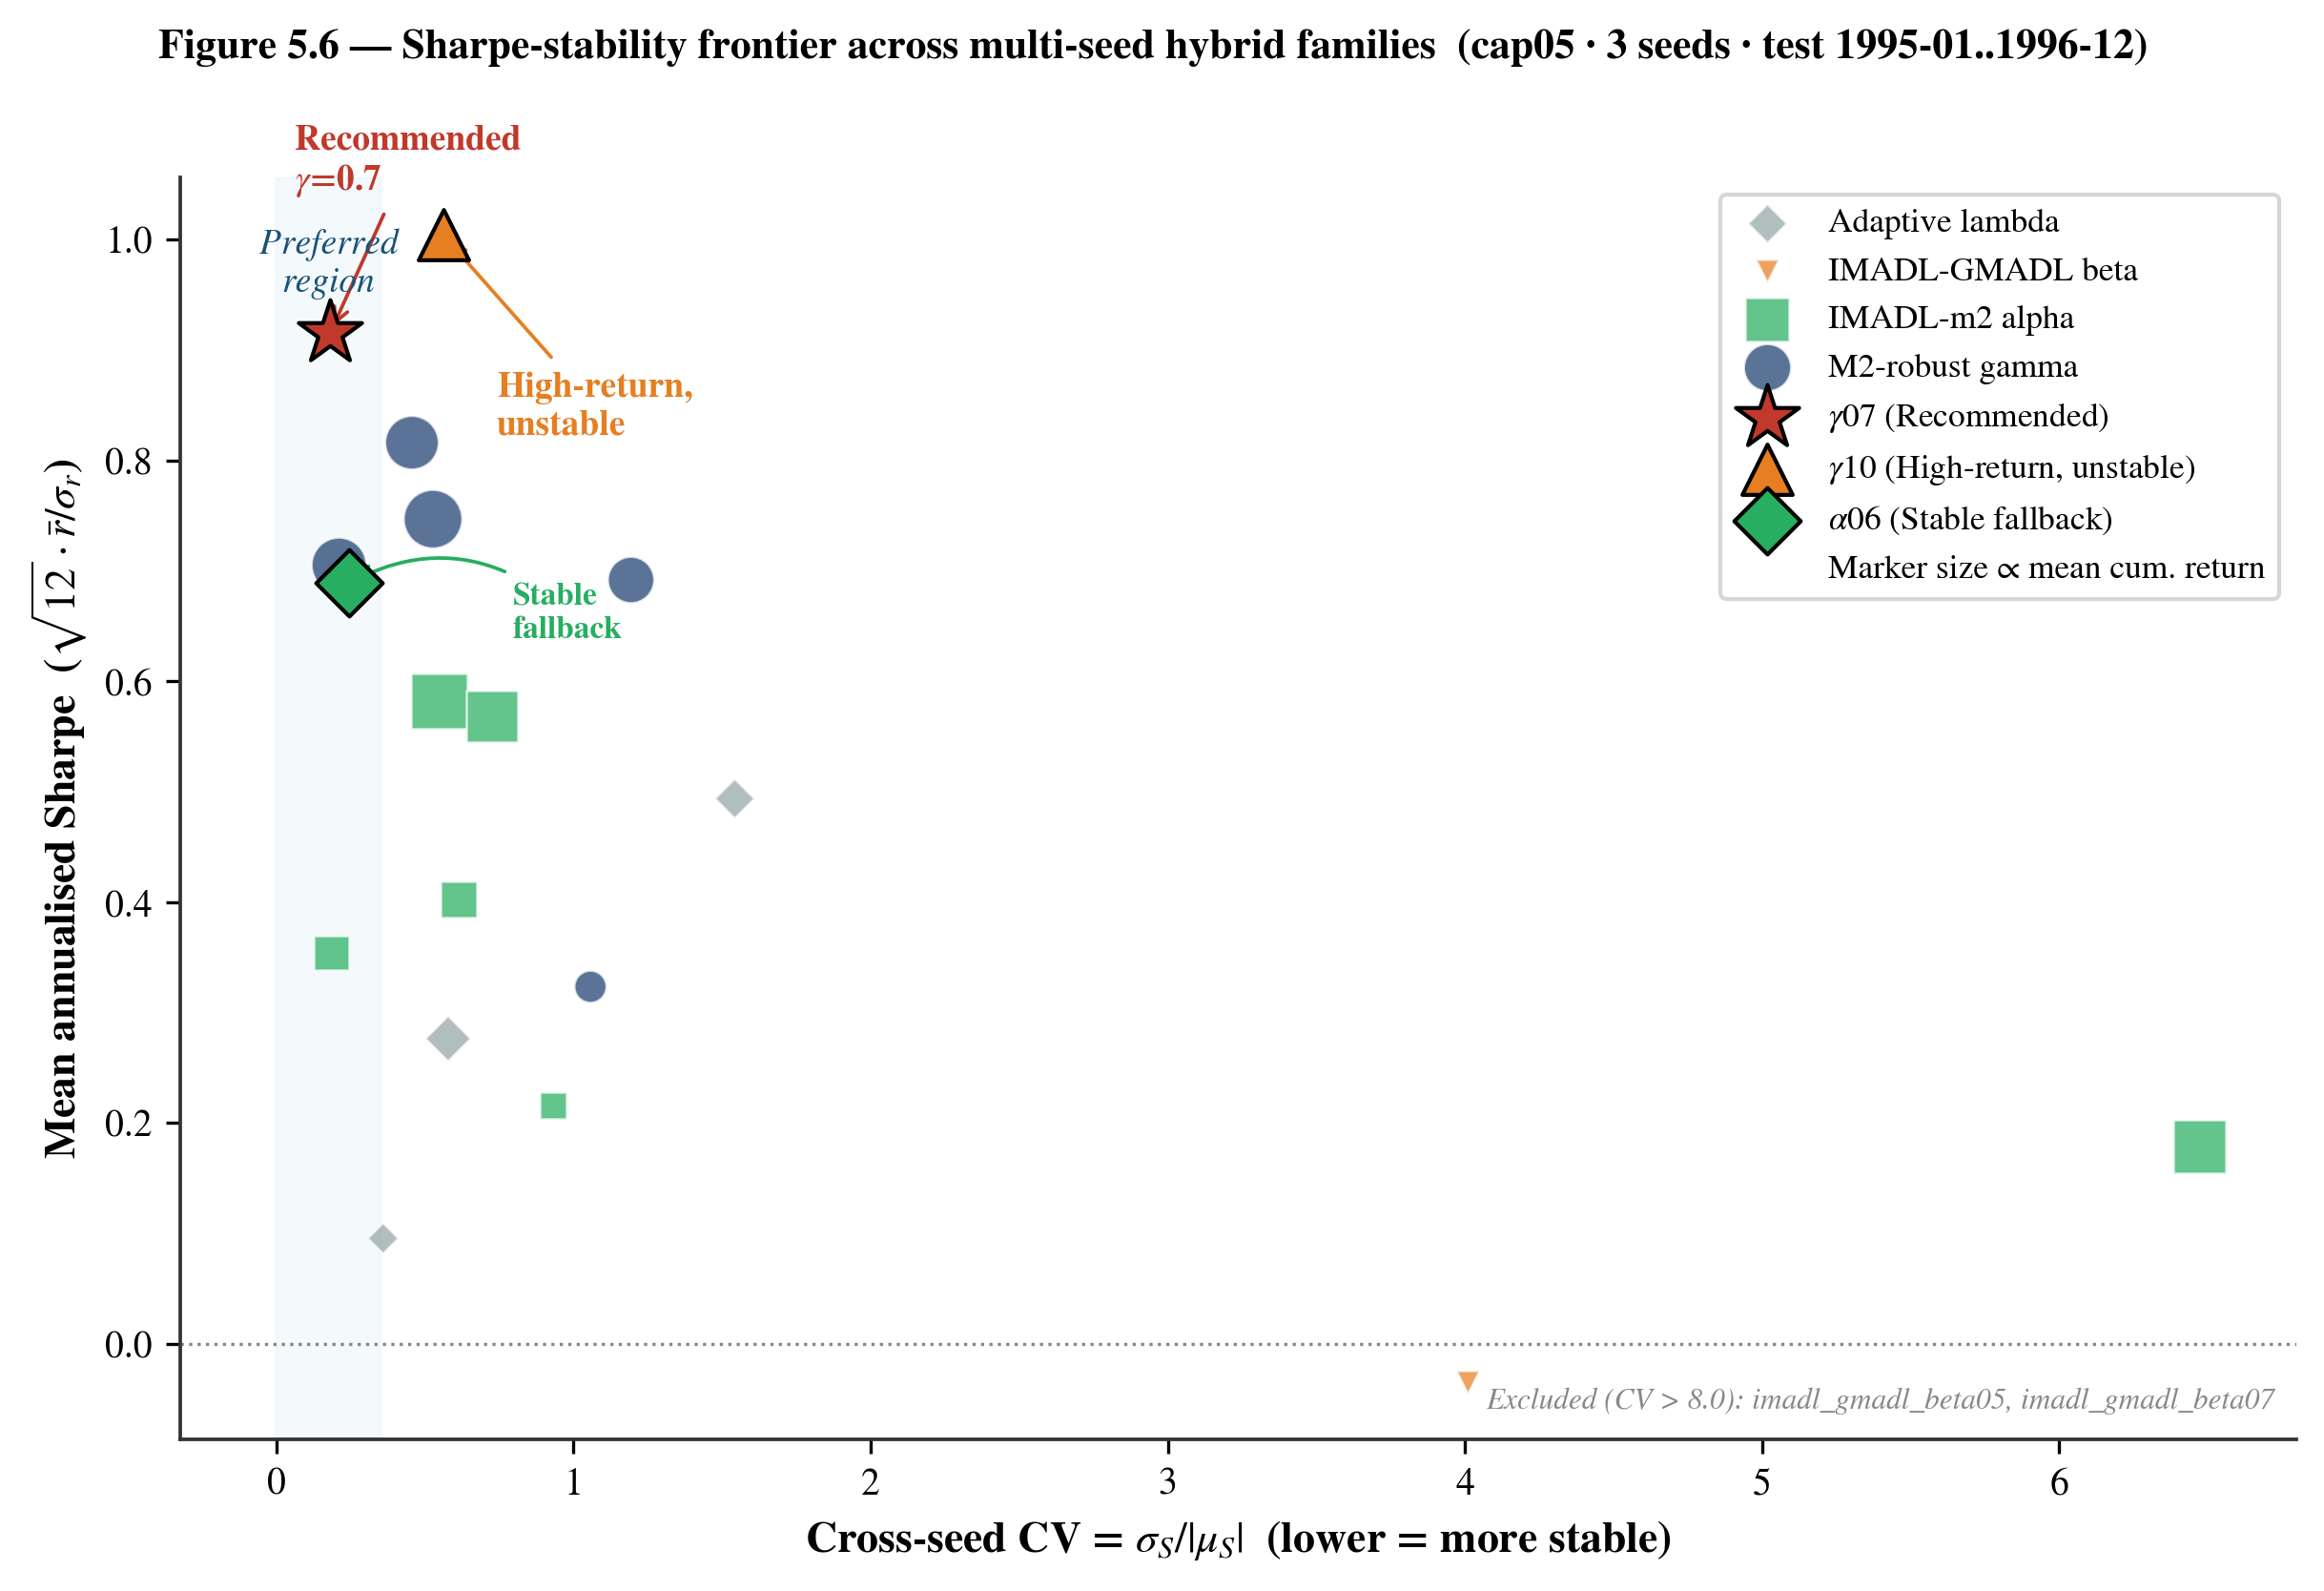
\includegraphics[width=0.9\textwidth]{figures/fig5_6_sharpe_cv_frontier.png}
\caption[Sharpe-stability frontier across multi-seed hybrid families]{Sharpe-stability frontier across multi-seed hybrid families. Each point is a 3-seed grouped summary. x-axis: cross-seed CV (lower = more stable); y-axis: mean annualised Sharpe; marker size proportional to mean cumulative return. Blue shading marks the preferred region (CV $\leq 0.35$). Red star: \texttt{m2\_robust\_gamma07} (recommended); orange triangle: \texttt{m2\_robust\_gamma10}; green diamond: \texttt{imadl\_m2\_alpha06} (stable fallback). Rows with CV $> 8$ (IMADL-GMADL $\beta$07) are excluded and noted in the figure. Evaluation window \texttt{1995-01..1996-12}, \texttt{cap05}, 3 seeds per row.}
\label{fig:sharpe-cv-frontier}
\end{figure}

\section{Phase 4: Loss-component normalisation probe}

\label{sec:phase4-normalisation-probe}

A natural concern with the hybrid-multiplicative design is that the directional-prediction term and the error-magnitude term operate on different scales, and that the observed Sharpe differences might simply reflect scale imbalance rather than genuine loss-family differences. The normalisation probe runs a component-level normalisation on the three candidate variants (\texttt{m2\_robust\_gamma07}, \texttt{m2\_robust\_gamma10}, \texttt{imadl\_m2\_alpha06}) to test whether equalising the scale of the two terms materially changes the ranking.

Table~\ref{tab:normalisation-probe} summarises the probe. The scale ratios quoted are estimated from Phase~3 diagnostics; as the probe's own summary records, a fully instrumented per-component logger has not yet been implemented, so the ratios should be treated as diagnostics-grade rather than fully measured.

\begin{table}[H]
\centering
\caption{Loss-component normalisation probe. Static train \texttt{1990-01..1994-12}, test \texttt{1995-01..1996-12}, \texttt{cap05}, 3 seeds per row. Source: see Appendix~B \SB.4.}
\label{tab:normalisation-probe}
\begin{tabular}{ccccc}
\toprule
Loss & Scale ratio & Original & Normalised & Normalised per-seed \\
& (dir.\ vs MSE) & mean Sharpe & mean Sharpe & Sharpes \\
\midrule
\texttt{m2\_robust\_gamma07} & $\sim 113$ & $0.9156$ & $0.9112$ & $0.5956, 1.4064, 0.7317$ \\
\texttt{m2\_robust\_gamma10} & $\sim 113$ & $1.0043$ & $0.4072$ & $0.6254, 0.1181, 0.4780$ \\
\texttt{imadl\_m2\_alpha06} & $\sim 34$ & $0.6895$ & $-0.0161$ & $0.5628, -0.8335, 0.2224$ \\
\bottomrule
\end{tabular}
\end{table}

\begin{figure}[H]
\centering
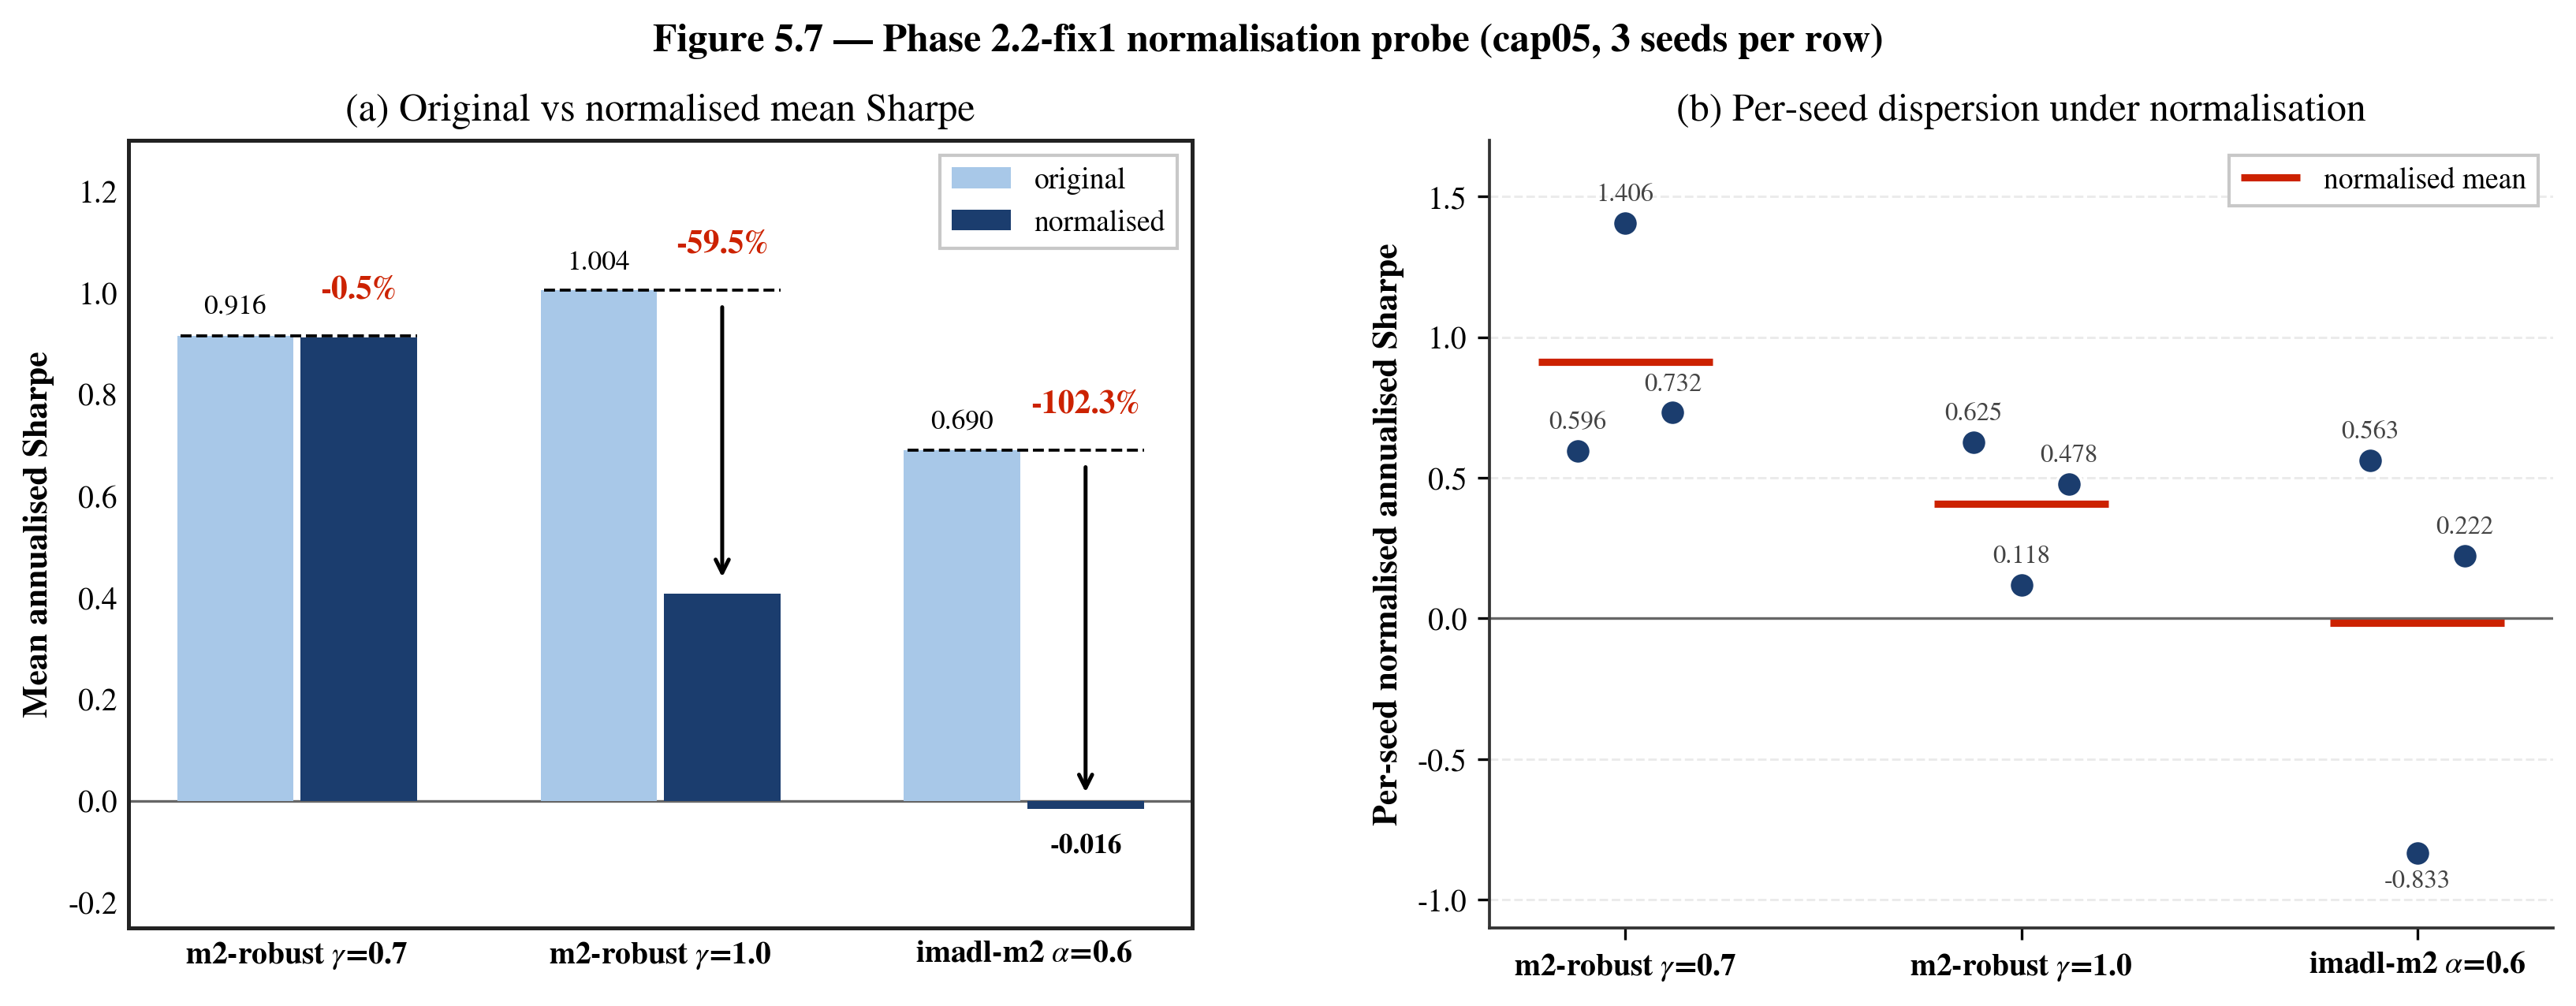
\includegraphics[width=0.9\textwidth]{figures/fig5_7_normalisation_probe.png}
\caption[Loss-component normalisation probe]{Loss-component normalisation probe. Left: grouped bar showing the original vs normalised mean annualised Sharpe for the three strongest candidates (\texttt{m2\_robust\_gamma07}, \texttt{m2\_robust\_gamma10}, \texttt{imadl\_m2\_alpha06}), 3 seeds per row. Right: per-seed normalised Sharpes (dots) and their mean (short horizontal bar) for each candidate. Evaluation window \texttt{1995-01..1996-12}, \texttt{cap05}. Scale ratios are diagnostics-estimated (per-component logger not yet implemented).}
\label{fig:normalisation-probe}
\end{figure}

Three points follow. First, normalisation is not a universal fix. Only \texttt{gamma07} is approximately stable under normalisation (mean Sharpe moves from $0.9156$ to $0.9112$, a change smaller than the per-seed dispersion in either configuration). Both \texttt{gamma10} and \texttt{alpha06} degrade materially -- by roughly a factor of two for \texttt{gamma10} and to near zero for \texttt{alpha06}. Normalisation therefore does not correct scale imbalance in a uniform way.

Second, the fact that \texttt{gamma07} is approximately stable under the diagnostic normalisation probe while \texttt{gamma10} and \texttt{alpha06} are not suggests that the observed \texttt{gamma07} Sharpe is not an artefact of the specific relative scale of the two loss components. Its signal is consistent across the original and diagnostic-normalised settings. By contrast, \texttt{gamma10}'s apparent edge in mean Sharpe without normalisation is sensitive to scale and should be treated as a contingent result.

Third, the probe itself has a known limitation: the scale ratios are estimated from logged diagnostics rather than measured directly through a per-component logger. The probe is therefore consistent with -- but not dispositive of -- a design claim that \texttt{gamma07} is approximately scale-stable. Chapter~6 flags this as a priority for future work.

In summary, component normalisation is informative but is not recommended as a blanket fix across the hybrid-multiplicative family. \texttt{gamma07} does not require it; \texttt{gamma10} and \texttt{alpha06} are damaged by it in the current evidence.

\section{Claim-boundary diagnostics}

\label{sec:claim-boundary-diagnostics}

Diagnostic passes confirm that cross-phase comparisons (e.g., stacking Phase~2 tables against Phase~3 tables) involve small but systematic runner and formula differences that are not attributable to a single factor. These differences do not invalidate controlled comparisons within a single phase, but they prevent claims of the form ``Phase~3 improves Phase~2 by $X$ Sharpe points.''

Two claim boundaries follow. First, \textbf{intra-phase comparison is strong}: within each table the loss function is the only varying factor. Second, \textbf{inter-phase comparison is moderate to weak}: cross-phase comparisons differ in seed set, parameterisation, and implementation details (see \S3.8). They are reasonable as design motivation but should not be quoted as direct-improvement claims. The closest supportable cross-phase statement is descriptive: the $\gamma$ family, once evaluated under multi-seed conditions, produces a mean Sharpe that exceeds the best Phase~2 seed-42 variant, but the two rows differ in more than one experimental factor.

\section{Headline findings and recommendations}

\label{sec:headline-findings}

Figure~\ref{fig:cumulative-return-paths} shows the cumulative long-short return paths that underlie the summary statistics in \S5.2--\S5.5. The left panel places the Phase~1 baselines in time: MSE and IMADL produce negative or flat paths throughout the 24-month window, while the hybrid variants (M1, A3) accumulate positive returns steadily. The right panel shows the Phase~2 gamma robustness picture: \texttt{gamma07} (red) produces the most consistent upward path across all three seeds, with a narrow seed envelope; \texttt{gamma10} (orange) reaches a higher peak in its best seed but shows wider dispersion; \texttt{gamma03} collapses early and never recovers.

\begin{figure}[H]
\centering

\includegraphics[width=0.9\textwidth]{figures/fig5_8_cumulative_return_paths.png}
\caption[Cumulative long-short return paths]{Cumulative long-short return paths. Left: Phase~1 baseline losses at seed 42; solid lines for hybrid variants, dashed for pure directional losses. Right: Phase~2 M2-robust $\gamma$ sweep; thick line is the mean across 3 seeds and shaded band is the min--max seed envelope. Train \texttt{1990-01..1994-12}, test \texttt{1995-01..1996-12}, \texttt{cap05}.}
\label{fig:cumulative-return-paths}
\end{figure}

The final loss recommendation rests on \S5.4--\S5.6, which together constitute the only multi-seed robustness evidence reported in this chapter. The recommendation has three tiers:

\textbf{Primary: \texttt{m2\_robust\_gamma07}.} Mean Sharpe $0.9156$, coefficient of variation $0.1808$, mean cumulative return $+27.99\%$ over 24 months, evaluated across three seeds on the \texttt{cap05} portfolio. Approximately stable under the diagnostic normalisation probe (normalised mean Sharpe $0.9112$). No seed in the run produces a negative Sharpe. This is the best-supported single choice for a loss function in the design space studied in this report.

\textbf{High-return alternative: \texttt{m2\_robust\_gamma10}.} Mean Sharpe $1.0043$ is the highest in the integrated sweep, but its coefficient of variation $0.5613$ is three times that of \texttt{gamma07}, its per-seed Sharpe range is wide ($0.4587$ to $1.5847$), and normalisation reduces its mean Sharpe to $0.4072$. It is appropriate only where the reader knowingly accepts high seed-sensitivity in exchange for a higher best-case Sharpe.

\textbf{Stable fallback: \texttt{imadl\_m2\_alpha06}.} Mean Sharpe $0.6895$, CV $0.2443$, mean cumulative return $+30.42\%$. This is the peak of the IMADL-m2 $\alpha$ sweep and its cumulative return is actually the largest of the three tiered candidates, though its Sharpe is lower than \texttt{gamma07}. It is selected as the stable fallback by its favourable stability/return trade-off rather than by Sharpe dominance, and it provides the next-best independent corroboration that a hybrid-multiplicative design with a robust component is the productive region of the loss space.

In summary, the empirical answer to the research questions posed in Chapter~1 is: within the static 24-month protocol studied here, a hybrid-multiplicative loss with a tuned robust component ($\gamma = 0.07$) outperforms traditional regression losses and pure absolute-loss variants on seed-42 same-window Sharpe, and among the competitive Phase~2 multi-seed rows it achieves the best joint Sharpe-stability profile, with a stable fallback available through the IMADL-m2 $\alpha$ family at the same order of Sharpe. Scope limitations are discussed in Chapter~6.
